\section{Introduction}
%
%  Introduction
%
\begin {frame} {Path Planning}
  Given
  \begin{itemize}
  \item A robot (kinematic chain),
  \pause
  \item obstacles,
  \pause
  \item constraints (non-holonomic, manipulation),
  \pause
  \item an initial configuration and
  \item goal configurations,
\end{itemize}
  \pause
  Compute a collision-free path satisfying the constraints from the initial
  configuration to a goal configuration.
\end {frame}

%
%  Historical perspective
%

\begin {frame} {Historical perspective}
  \begin{itemize}
    \item 1998: Move3D,
      \pause
    \item 2001: Creation of Kineo-CAM, transfer of Move3D,
      \pause
    \item 2006: Release of KineoWorks-2, development of HPP based on KineoWorks-2,
      \pause
    \item 2013: kineo-CAM is bought by Siemens,
      \pause
    \item December 2013: development of HPP open-source.
  \end{itemize}
\end {frame}

%
%  Main features
%

\begin {frame} {Main features}
  \begin {itemize}
  \item Numerical constraints at the core of the model
    \begin {itemize}
    \item quasi-static equilibrium
    \item object grasp and placement
    \item explicit and implicit constraints
    \end {itemize}
    \pause
  \item no a priori discretization of paths
    \begin {itemize}
    \item evaluation calls constraint projection
    \item constrained path need to be checked for continuity (class \texttt{hpp::core::PathProjector})
    \end {itemize}
  \end {itemize}
\end{frame}

\section {Description of the software}

%
%  Overview of the architecture
%

\begin {frame} {Overview of the architecture}
  Modular: collection of packages
  \pause
  \begin{itemize}
    \item package dependencies tracked by \texttt{pkg-config},
      \pause
    \item installation managed by \texttt{cmake} and a \texttt{git}
      submodule: {\tiny\texttt{git://github.com/jrl-umi3218/jrl-cmakemodules.git}},
      \pause
    \item programmed in \texttt{C++},
      \pause
    \item controlled via \texttt{python}
  \end{itemize}
\end {frame}


%
%  Overview of the architecture
%

\begin {frame} {Overview of the architecture}
\parbox {\linewidth} {
  \centerline {
    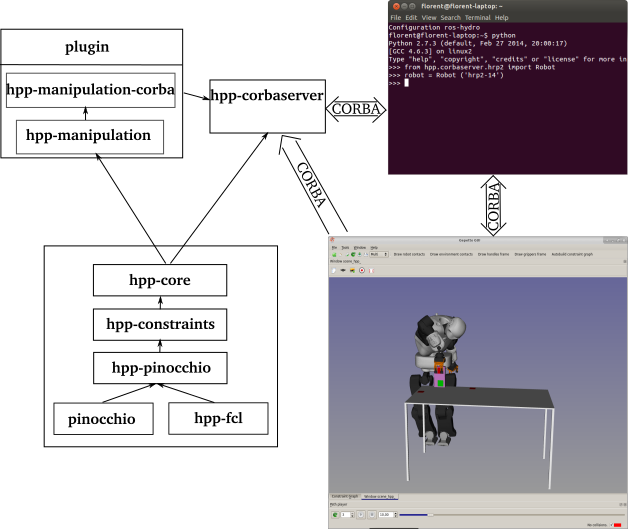
\includegraphics[width=.6\linewidth]{figures/archi-hpp.png}
  }
}
\end {frame}

%
%  HPP SDK
%

\begin {frame} {Software Development Kit}

Packages implementing the core infrastructure
\begin{itemize}
\item Kinematic chain with geometry
  \begin{itemize}
  \item \texttt{pinocchio}: implementation of kinematic chain with geometry,
    \begin{itemize}
      \item tree of joints (Rotation, Translation, SE3: vector + unit-quaternions),
      \item moving fcl::CollisionObjects,
      \item forward kinematics,
      \item joint Jacobians,
      \item center of mass and Jacobian,
      \item URDF parser.
    \end{itemize}
  \end{itemize}
  \pause
\item Numerical constraints
  \begin{itemize}
  \item \texttt{hpp-constraints}: numerical constraints
    \begin {itemize}
    \item implicit $f (\conf) = (\leq) 0$,
    \item explicit $\conf_{out} = f (\conf_{in})$,
    \item numerical solvers based on Newton-Raphson.
    \end{itemize}
  \end{itemize}
\end{itemize}
\end {frame}

\begin {frame} {Newton-Raphson algorithm}
  \parbox {.5\linewidth} {
    \centerline {
      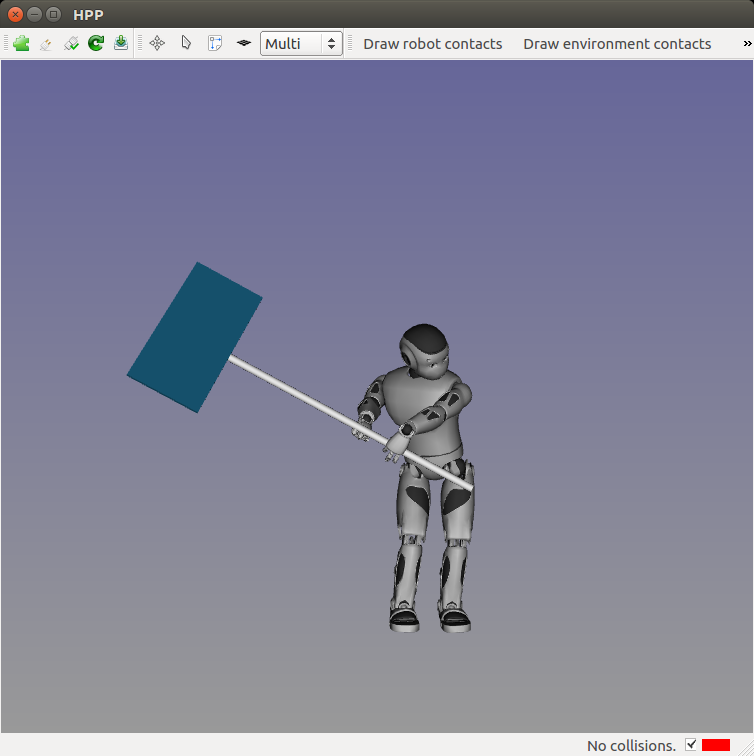
\includegraphics [width=\linewidth] {figures/seq/romeo-7.png}
    }
  }
  \hspace*{.05\linewidth}
  \parbox {.39\linewidth} {
    Constraints
    \begin {itemize}
    \item quasi-static equilibrium (15)
    \item both hands hold the placard (10)
    \end{itemize}
  }
  \centerline {
    Goal: Generate a configuration satisfying the constraints.
  }
\end {frame}

\begin {frame} {Newton-Raphson algorithm}
  \parbox {.5\linewidth} {
    \centerline {
      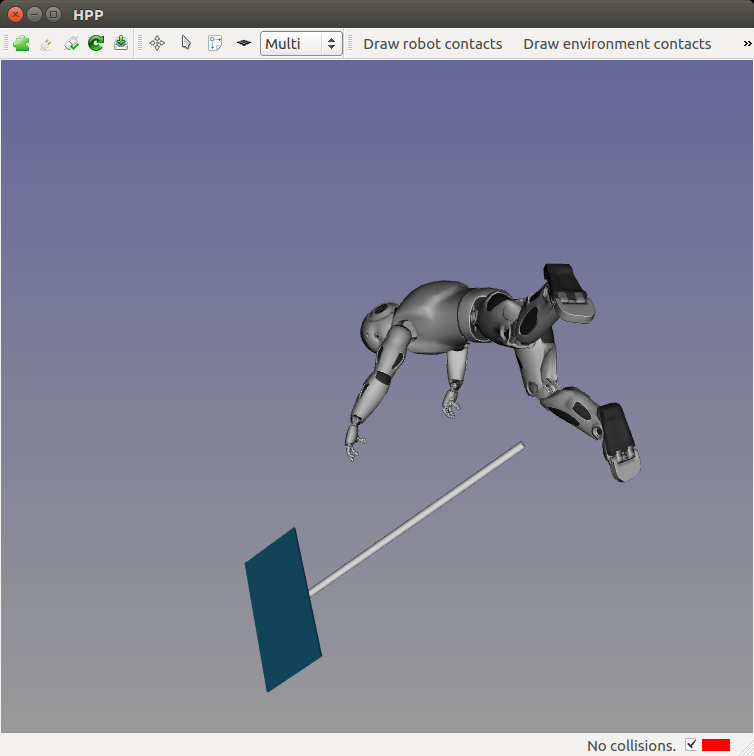
\includegraphics [width=\linewidth] {figures/seq/romeo-0.png}
    }
  }
  \hspace*{.05\linewidth}
  \parbox {.39\linewidth} {
    Constraints
    \begin {itemize}
    \item quasi-static equilibrium (15)
    \item both hands hold the placard (10)
    \end{itemize}
  }
  \centerline {
    Shoot random configuration
  }
\end {frame}

\begin {frame} {Newton-Raphson algorithm}
  \parbox {.5\linewidth} {
    \centerline {
      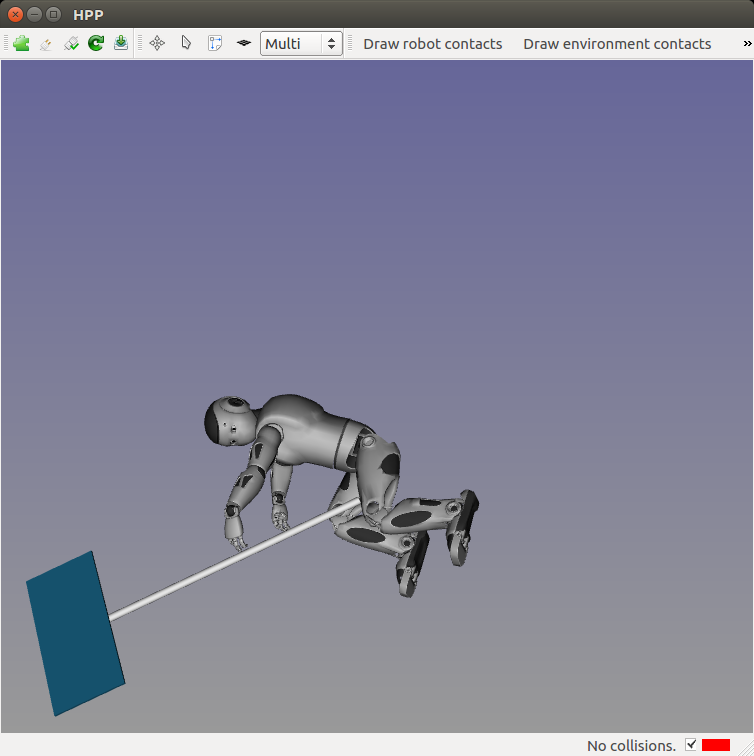
\includegraphics [width=\linewidth] {figures/seq/romeo-1.png}
    }
  }
  \hspace*{.05\linewidth}
  \parbox {.39\linewidth} {
    Constraints
    \begin {itemize}
    \item quasi-static equilibrium (15)
    \item both hands hold the placard (10)
    \end{itemize}
  }
  \centerline {
    Solve linearized system
  }
\end {frame}

\begin {frame} {Newton-Raphson algorithm}
  \parbox {.5\linewidth} {
    \centerline {
      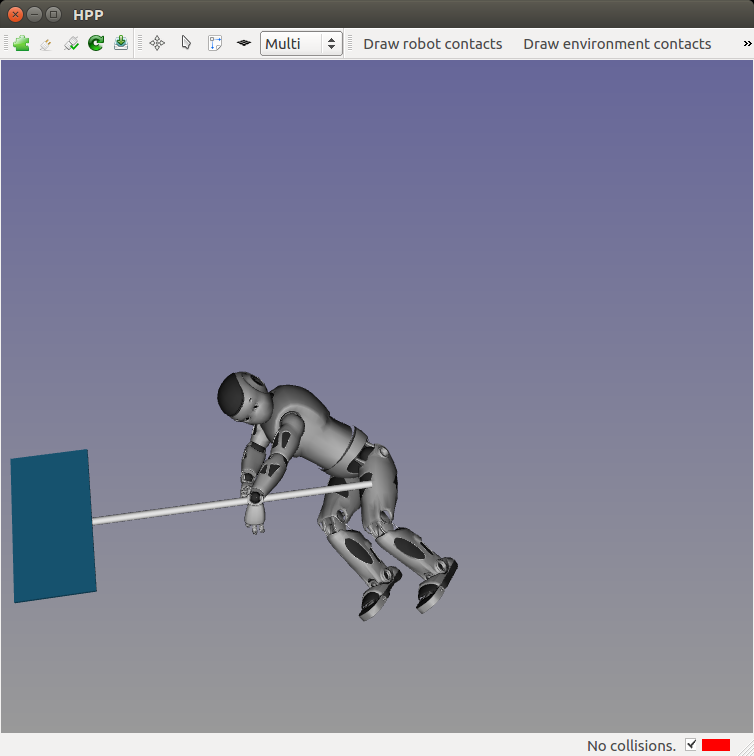
\includegraphics [width=\linewidth] {figures/seq/romeo-2.png}
    }
  }
  \hspace*{.05\linewidth}
  \parbox {.39\linewidth} {
    Constraints
    \begin {itemize}
    \item quasi-static equilibrium (15)
    \item both hands hold the placard (10)
    \end{itemize}
  }
  \centerline {
    Solve linearized system
  }
\end {frame}

\begin {frame} {Newton-Raphson algorithm}
  \parbox {.5\linewidth} {
    \centerline {
      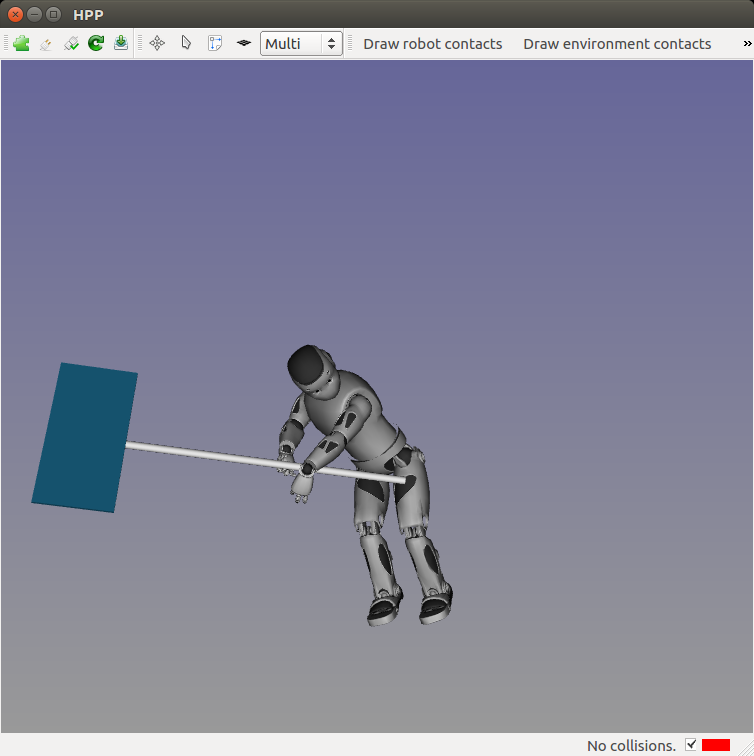
\includegraphics [width=\linewidth] {figures/seq/romeo-3.png}
    }
  }
  \hspace*{.05\linewidth}
  \parbox {.39\linewidth} {
    Constraints
    \begin {itemize}
    \item quasi-static equilibrium (15)
    \item both hands hold the placard (10)
    \end{itemize}
  }
  \centerline {
    Solve linearized system
  }
\end {frame}

\begin {frame} {Newton-Raphson algorithm}
  \parbox {.5\linewidth} {
    \centerline {
      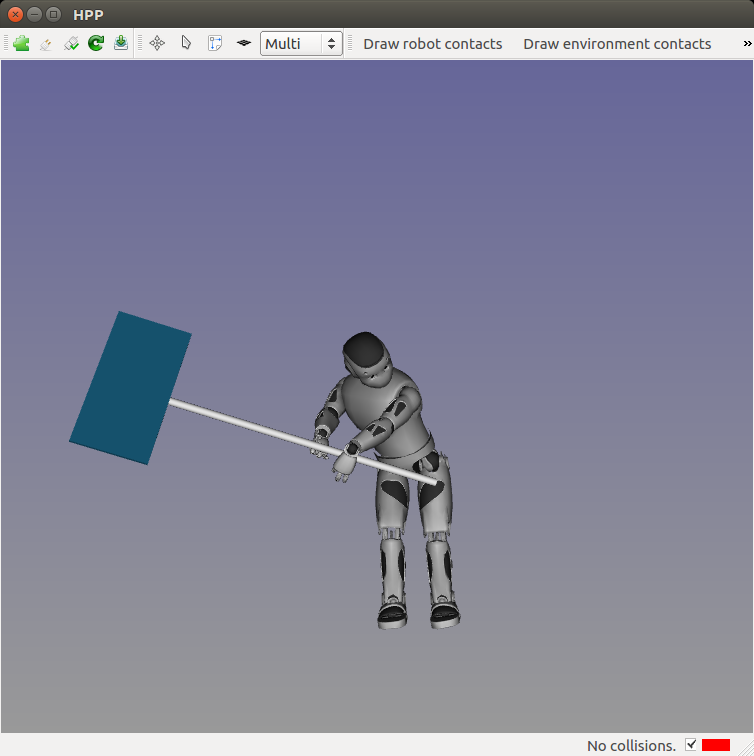
\includegraphics [width=\linewidth] {figures/seq/romeo-4.png}
    }
  }
  \hspace*{.05\linewidth}
  \parbox {.39\linewidth} {
    Constraints
    \begin {itemize}
    \item quasi-static equilibrium (15)
    \item both hands hold the placard (10)
    \end{itemize}
  }
  \centerline {
    Solve linearized system
  }
\end {frame}

\begin {frame} {Newton-Raphson algorithm}
  \parbox {.5\linewidth} {
    \centerline {
      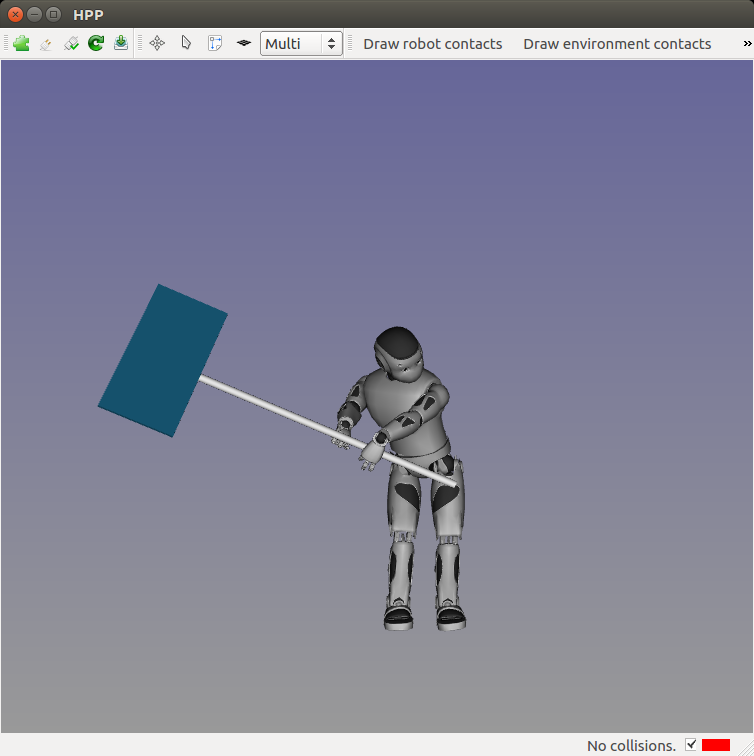
\includegraphics [width=\linewidth] {figures/seq/romeo-5.png}
    }
  }
  \hspace*{.05\linewidth}
  \parbox {.39\linewidth} {
    Constraints
    \begin {itemize}
    \item quasi-static equilibrium (15)
    \item both hands hold the placard (10)
    \end{itemize}
  }
  \centerline {
    Solve linearized system
  }
\end {frame}

\begin {frame} {Newton-Raphson algorithm}
  \parbox {.5\linewidth} {
    \centerline {
      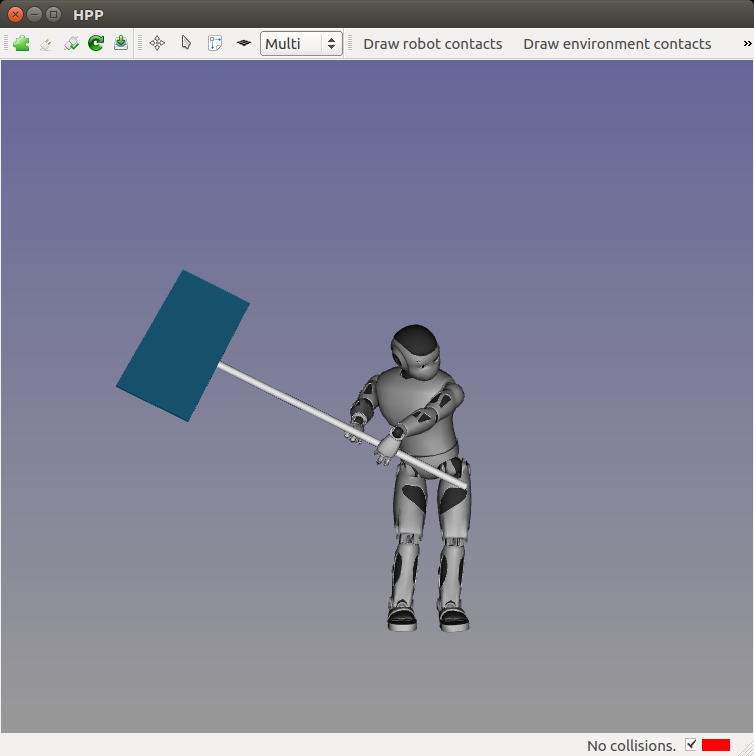
\includegraphics [width=\linewidth] {figures/seq/romeo-6.png}
    }
  }
  \hspace*{.05\linewidth}
  \parbox {.39\linewidth} {
    Constraints
    \begin {itemize}
    \item quasi-static equilibrium (15)
    \item both hands hold the placard (10)
    \end{itemize}
  }
  \centerline {
    Solve linearized system
  }
\end {frame}

\begin {frame} {Newton-Raphson algorithm}
  \parbox {.5\linewidth} {
    \centerline {
      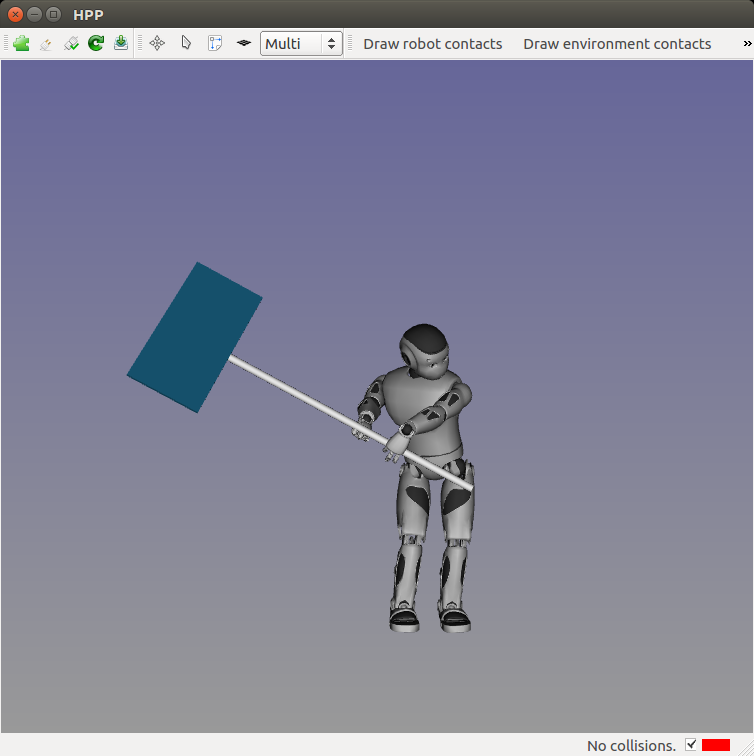
\includegraphics [width=\linewidth] {figures/seq/romeo-7.png}
    }
  }
  \hspace*{.05\linewidth}
  \parbox {.39\linewidth} {
    Constraints
    \begin {itemize}
    \item quasi-static equilibrium (15)
    \item both hands hold the placard (10)
    \end{itemize}
  }
  \centerline {
    Result: a configuration that satisfies the constraints.
  }
\end {frame}

\begin {frame} {Software Development Kit}

Packages implementing the core infrastructure
\begin{itemize}
\item Path planning
  \begin{itemize}
  \item \texttt{hpp-core}: definition of basic classes,
    \begin{itemize}
      \item path planning problems,
      \item path planning solvers (RRT),
      \item constraints (locked dofs, numerical constraints)
      \item path optimizers (random shortcut),
      \item steering methods (straight interpolation)
    \end{itemize}
  \end{itemize}
\end{itemize}
\end {frame}


\begin {frame} {Extensions}

Packages implementing other algorithms
\begin{itemize}
  \item \texttt{hpp-wholebody-step}: whole-body and walk planning using sliding path approximation,
    \pause
  \item \texttt{hpp-manipulation}: manipulation planning (see next section),
    \pause
  \item any extension for a given application.
\end{itemize}
\end {frame}

%
%  Python control
%

\begin {frame} {Python control}

\texttt{hpp-corbaserver}: python scripting through CORBA
\begin{itemize}
\item embed \texttt{hpp-core} into a CORBA server and expose services through 3 \texttt{idl} interfaces:
  \begin{itemize}
  \item \texttt{Robot} load and initializes robot,
  \item \texttt{Obstacle} load and build obstacles,
  \item \texttt{Problem} define and solve problem.
  \end{itemize}
\pause
\item Implement python classes to help user call CORBA services
  \begin{itemize}
    \item \texttt {Robot} automatize robot loading,
    \item \texttt {ProblemSolver} definition problem helper.
  \end{itemize}
\end{itemize}
\end {frame}

%
%  Python control
%

\begin {frame} {Python control}
  Extensions through plugins in \texttt{hpp-corbaserver}
  \begin{itemize}
    \item \texttt {hpp-manipulation-corba:} control of manipulation planning specific classes and algorithms.
  \end{itemize}
\end {frame}

%
%  Visualization through ROS/rviz
%

\begin {frame} {Visualization through gepetto-gui}
  \begin{center}
    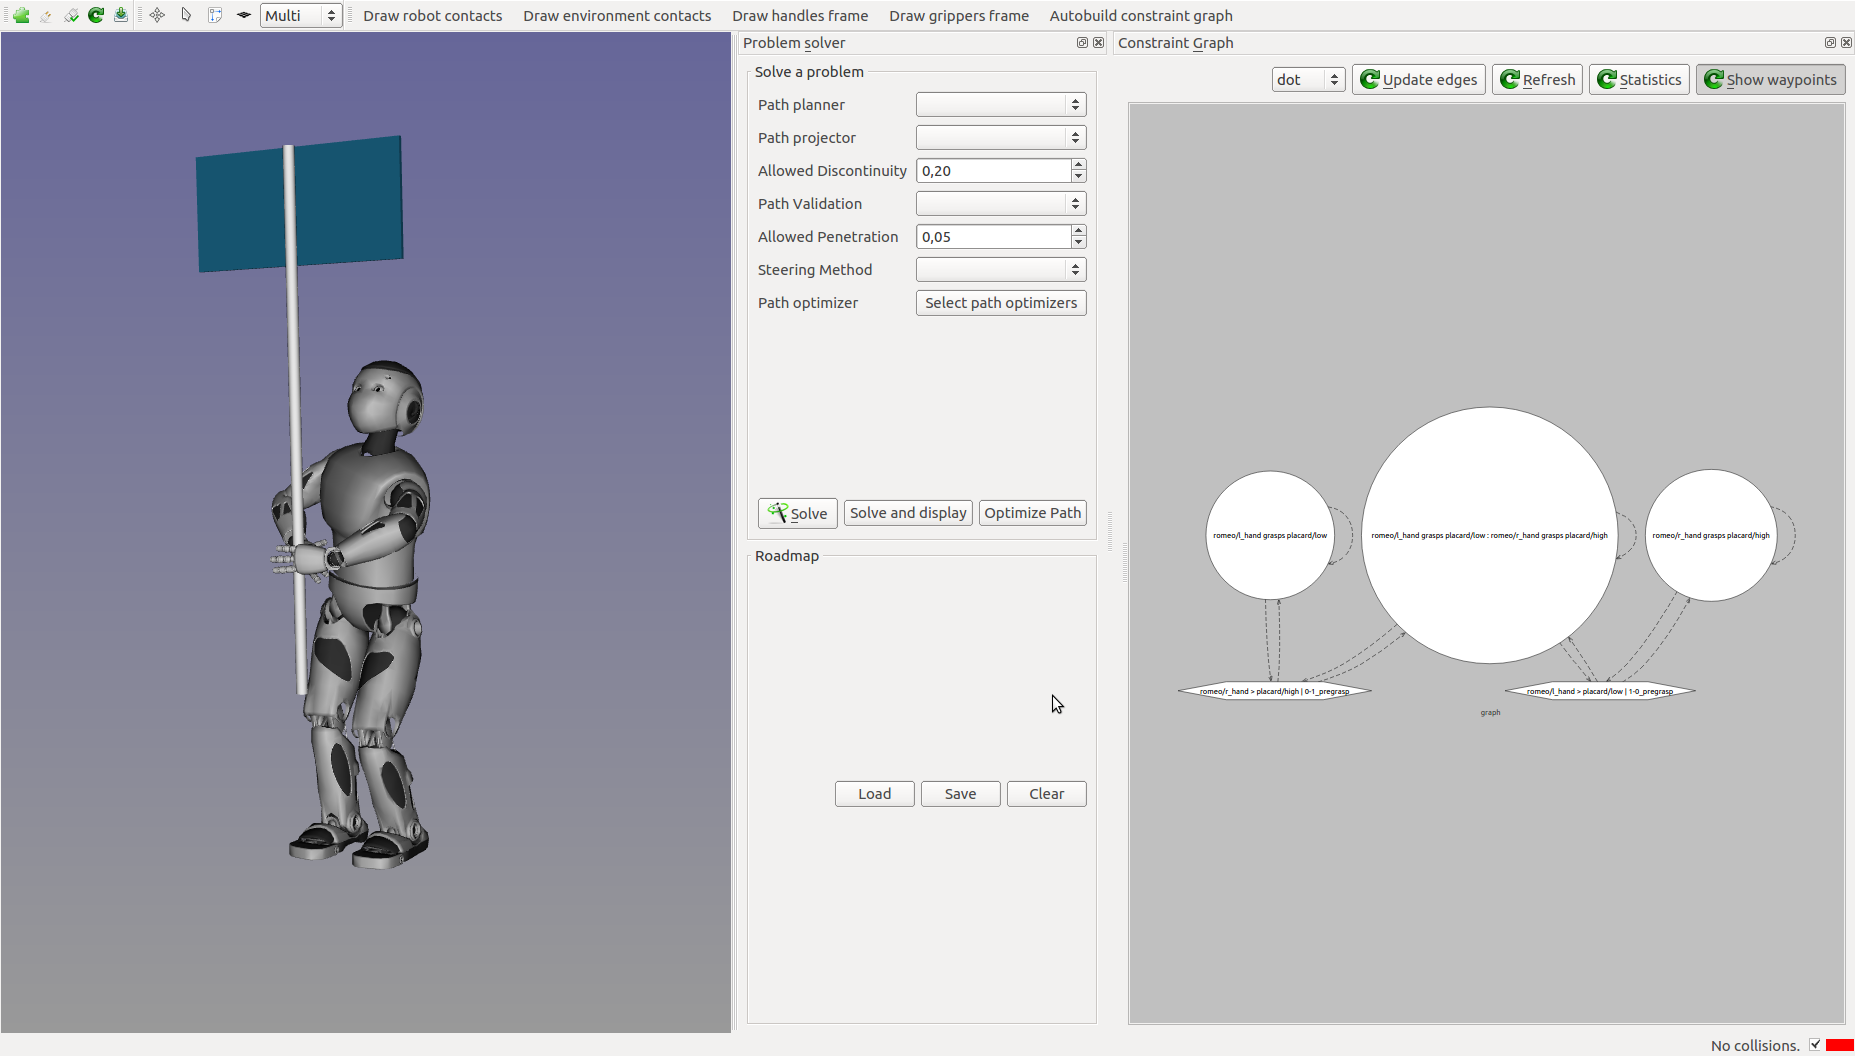
\includegraphics [width=.9\linewidth] {figures/gepetto-gui.png}
  \end{center}
  Implemented by package \texttt {hpp-gepetto-viewer}.
\end {frame}

\section {Manipulation planning}

%
%  Manipulation
%

\begin {frame} {Manipulation}
  Class of problem containing:
  \begin{itemize}
    \item A robot: actuated DOFs
    \item Objects: unactuated DOFs
  \end{itemize}
  \pause
  A solution will be a succession of motion of two types:
  \begin{itemize}
    \item The robot moves without constraints. Objects do not move.
    \item The robot moves while grasping the object.
  \end{itemize}
\end {frame}

\begin {frame} {Manipulation}
  \only<1>{2 states:}
  \only<2->{4 transitions:}
  \begin{figure}
    \centering
    \begin{tikzpicture}[>=stealth',auto,node distance=3cm,
      thick,main node/.style={circle,draw,text width=1.7cm,align=center,font=\footnotesize}]
      \setbeamercovered{transparent}
      \node[main node] (nh) {Not holding};
      {\visible<2->{\uncover<2,4->{\path[->] (nh) edge[loop left] node[left, text width=1.2cm, align=right] {Object fixed} (nh);}}}

      \node[main node] (h) [right of=nh] {Holding};
      {\visible<2->{\uncover<2,4->{\path[<-] (h) edge[bend right=45] node[above] {Grasp} (nh);}}}
      {\visible<2->{\uncover<3->{\path[->] (h) edge[bend left=45] node[below] {Ungrasp} (nh);}}}
      {\visible<2->{\uncover<3->{\path[->] (h) edge[loop right] node[right, text width=1.7cm] {Keep the grasp} (h);}}}
    \end{tikzpicture}
    \label{fig:graphEEAndObject}
  \end{figure}
\end {frame}

\begin{frame}{Constraint}
  \uncover<1->{
    \begin{block}{Definition}
      A function $f \in D^1(\mathcal{C}, \mathbb{R}^m)$.
    \end{block}
  }
  \uncover<2->{
    \begin{exampleblock}{Foliation}
      A leaf of a constraint $f$ is defined by:
      $$ L_{f_0}(f) = \left\{\conf \in \mathcal{C} | f(\conf) = f_0 \right\} $$
    \end{exampleblock}
    where $f_0$ is called the \textit{right hand side} of the constraint.
  }
  \uncover<3->{
    \begin{alertblock}{Projection}
      Using a Newton Descent algorithm:
      $$ \conf_{rand} | f(\conf_{rand}) \ne f_0 \Rightarrow \conf_{proj} | f(\conf_{proj}) = f_0 $$
    \end{alertblock}
  }
\end{frame}

\begin{frame}{Constraint}
  Two types of constraints:
  \begin{block}{Configuration}
    Only one leaf is interesting: $L_{0} (f)$.
  \end{block}
  \begin{block}{Motion}
    A leaf also represents reachability space.
  \end{block}
\end{frame}

\begin{frame}{Foliation}
  In the configuration space:

  \begin{columns}
    \column{0.4\textwidth}
    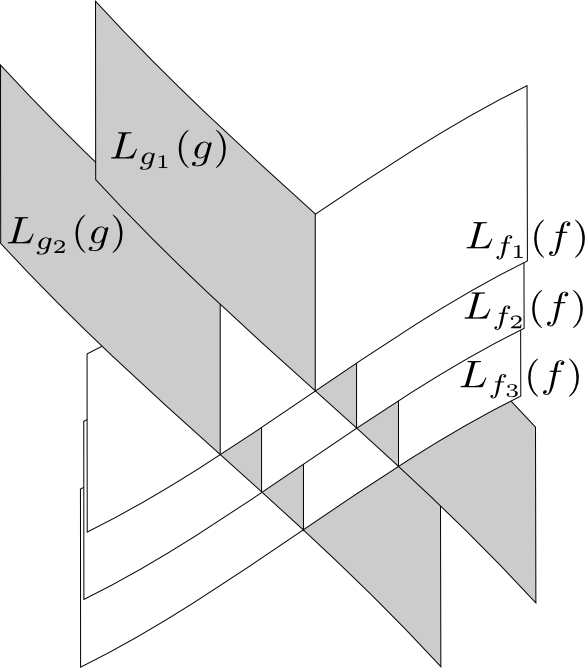
\includegraphics[width=1\textwidth,height=1\textheight,keepaspectratio]{figures/foliation.png}
    \column{0.6\textwidth}
    \begin{block}{2 constraints on motion}
      \begin{itemize}
        \item $f$: position of the object.
        \item $g$: grasp of the object.
      \end{itemize}
    \end{block}
  \end{columns}
\end{frame}

\begin{frame}{Constraint graph}
  \begin{columns}
    \column{0.5\textwidth}
    \only<1> {
      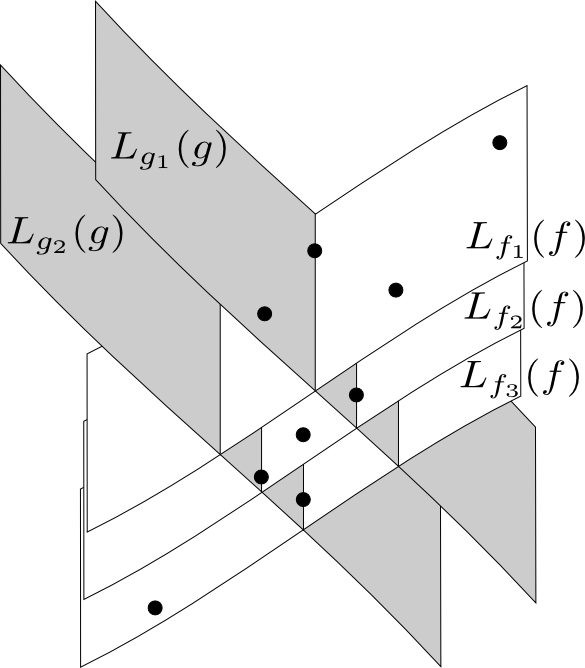
\includegraphics[width=0.9\textwidth,height=0.9\textheight,keepaspectratio]{figures/foliation_path1.png}
    }
    \only<2-> {
      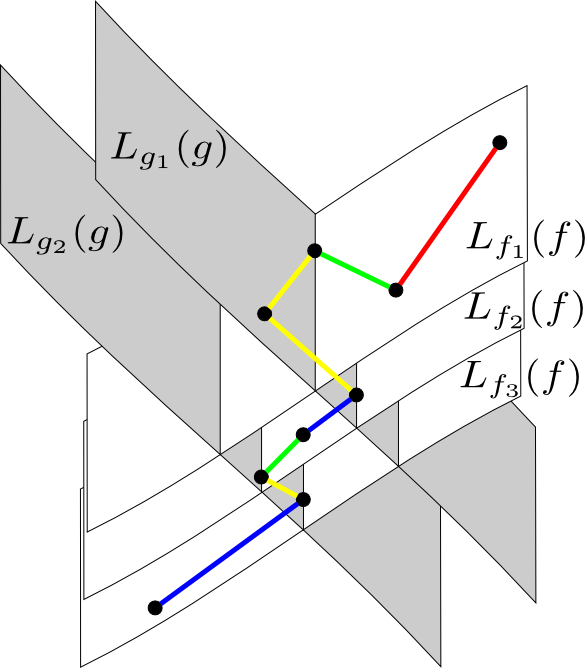
\includegraphics[width=0.9\textwidth,height=0.9\textheight,keepaspectratio]{figures/foliation_path2.png}
    }
    \column{0.5\textwidth}
    \centering
    \begin{tikzpicture}[>=stealth',auto,node distance=1.5cm,
      thick,main node/.style={circle,draw,text width=0.5cm,align=center,font=\footnotesize}]
      \setbeamercovered{transparent}
      \node[main node] (nh) {$L_f$};
      {\visible<2->{\path[->] (nh) edge[loop left, red] node[left, align=right] {f} (nh);}}

      \node[main node] (h) [right of=nh] {$L_g$};
      {\visible<2->{\path[<-] (h) edge[bend right=45, green] node[above] {f} (nh);}}
      {\visible<2->{\path[->] (h) edge[bend left=45, blue] node[below] {f} (nh);}}
      {\visible<2->{\path[->] (h) edge[loop right, yellow] node[right] {g} (h);}}
    \end{tikzpicture}
  \end{columns}
\end{frame}

\begin{frame}[fragile]{Rapidly exploring Random Tree}
  \begin{columns}
    \column{0.4\textwidth}
    \includegraphics<1>  [width=\textwidth,height=\textheight,keepaspectratio]{figures/seq/foliation-project-seq-1.png}
    \includegraphics<2-3>[width=\textwidth,height=\textheight,keepaspectratio]{figures/seq/foliation-project-seq-2.png}
    \includegraphics<4>  [width=\textwidth,height=\textheight,keepaspectratio]{figures/seq/foliation-project-seq-3.png}
    \includegraphics<5>  [width=\textwidth,height=\textheight,keepaspectratio]{figures/seq/foliation-project-seq-4.png}
    \includegraphics<6>  [width=\textwidth,height=\textheight,keepaspectratio]{figures/seq/foliation-project-seq-5.png}
    \column{0.6\textwidth}
    \setbeamertemplate{itemize item}{}% Remove bullets frp, ote,oze sinote,
    \setlength\leftmargini{0em}
    \begin{itemize}[leftmargin=*]
      \item<1-> $\conf_{rand}$ = shoot\_random\_config()
      \item<2-> $\conf_{near}$ = nearest\_neighbor($\conf_{rand}$, $tree$)
      \item<3-> $f_e$, $f_p$ = select\_next\_state($\conf_{near}$)
      \item<4-> $\conf_{proj}$ = project($\conf_{rand}$, $f_e$)
      \item<5-> $\conf_{new}$ = extend($\conf_{near}$, $\conf_{proj}$, $f_p$)
      \item<6-> $tree$.insert\_node( ($\conf_{near}$, $\conf_{new}$, $f_p$) )
    \end{itemize}
  \end{columns}
\end{frame}

\begin{frame}{hpp-manipulation-corba}
  Provides tools to:
  \begin{itemize}
    \item read URDF files of robots and objects;
      \pause
    \item create grasp contraints between a end-effector (robot) and a handle (object);
      \pause
    \item build the graph of constraints;
  \end{itemize}
\end{frame}

%
%  Installation
%

\begin {frame} {Installation and documentation}
  Everything in
  {\scriptsize
    \href{https://humanoid-path-planner.github.io/hpp-doc}
         {\texttt {https://humanoid-path-planner.github.io/hpp-doc}}
  }
\end {frame}

%
%  Keep informed
%

\begin {frame} {Keep informed}
\begin{itemize}
\item Mailing list \texttt {hpp@laas.fr} to discuss issues related to the software,
\item github notifications for issues related to individual packages
\centerline {
  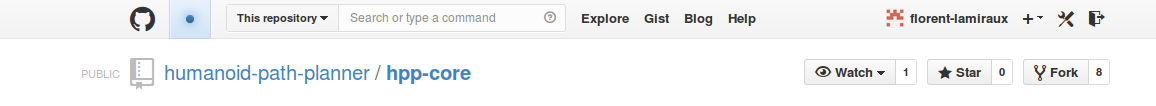
\includegraphics [width=\linewidth] {figures/github-watch.png}
}
\end{itemize}
\end {frame}

%
%  Perspectives
